\documentclass[11pt]{article}

\usepackage[a4paper, total={7in, 9.5in}]{geometry}
\usepackage{graphicx}
\usepackage{amssymb}
\usepackage{datetime}
\usepackage{pdfpages}
\usepackage{caption}
\usepackage{wrapfig}
\usepackage{tipa}
\usepackage{csvsimple}
\usepackage[T1]{fontenc}
\usepackage{hyperref}
\hypersetup{
	colorlinks=true,
	linkcolor=blue,
	filecolor=magenta,
	urlcolor=cyan,
	pdfpagemode=FullScreen,
}

\font\tenipa=tipa10
\def\schwa{{\tenipa\char64}}

\usepackage{array}
\newcolumntype{L}[1]{>{\raggedright\let\newline\\\arraybackslash\hspace{0pt}}p{#1}}
\newcolumntype{C}[1]{>{\centering\let\newline\\\arraybackslash\hspace{0pt}}p{#1}}
\newcolumntype{R}[1]{>{\raggedleft\let\newline\\\arraybackslash\hspace{0pt}}p{#1}}

\newdateformat{monthdayyeardate}{%
	\monthname[\THEMONTH]~\THEDAY, \THEYEAR}

\usepackage{setspace}
\usepackage{multirow}
\usepackage{xcolor}
\setlength{\parindent}{0em}
\setlength{\parskip}{0.5em}
\renewcommand{\baselinestretch}{1}

\begin{document}
\definecolor{myblue}{HTML}{3D4F7D}
\definecolor{myred}{HTML}{CD4F38}
\definecolor{mygreen}{HTML}{657060}
\definecolor{myorange}{HTML}{E48C2A}
\definecolor{mygreen2}{HTML}{44A57C}
\definecolor{myskyblue}{HTML}{64b5cd}

\makebox[0pt][l]{%
  \raisebox{-\totalheight}[0pt][0pt]{%
  
\includegraphics{media/uvic.jpg}
  }}%


\hspace*{\fill}\textbf{Earth \& Ocean Sciences 423 A01}\\
% (CRN 21332)
\hspace*{\fill}\textbf{UNIVERSITY OF VICTORIA}\\
\hspace*{\fill}\textbf{3-3-0 (1.5 UNITS)}\\
\hspace*{\fill}\textbf{SPRING TERM 2025}\\


\noindent\hrulefill

\begin{center}
\emph{We acknowledge and respect the L\schwa\'k$^w$\schwa ŋ\schwa n (Songhees and Esquimalt) Peoples on whose territory the university stands, and the L\schwa\'k$^w$\schwa ŋ\schwa n and WS\'ANE\'C Peoples whose historical relationships with the land continue to this day.}
\end{center}

\noindent\hrulefill

\begin{center}
\Large \textbf{COURSE OUTLINE}

\Large \textbf{EOS423: Advanced Sedimentology and Stratigraphy}

\normalsize Lectures: M/Th 1:00 to 2:20 PM in Clearihue A330 \\
\normalsize Labs: F 1:30 to 4:20 PM in Bob Wright Centre B119 \\
\end{center}

\noindent\hrulefill

\textbf{PREREQUISITES}: EOS201, 1 of EOS325 or EOS225\\
\textbf{COREQUISITES}: NONE\\

\textbf{CONTACT INFO}

\begin{center}
  \centering
  \begin{tabular}{ L{.25\linewidth}L{.25\linewidth}L{.25\linewidth} }
    Instructor(s):      & Blake Dyer &  \\
    Email:      & blakedyer@uvic.ca &  \\
    Office:      & BWC A419 &  \\
    Office Hours:      & by appointment &  \\
          &  &  \\
    Lab Coordinator      & Blake Dyer &  blakedyer@uvic.ca\\
Teaching Assistant(s)      & none &  \\
      &  &  \\
  \end{tabular}\\
\end{center}

\begin{center}
\textbf{COURSE DESCRIPTION}
\end{center}

In this course, we will explore how geologic and Earth surface processes, including tectonic, sea level and climate changes, are recorded and preserved in the stratigraphic record. Focus will be on modern and ancient case studies, with topics including basin analysis, cyclostratigraphy, process sedimentology and paleo-environmental reconstruction. Problem sets emphasize computational skills, including introductory time-series analysis, geospatial analysis and remote sensing.

The course will meet twice a week (M/Th) for lectures and on Fridays to work on the weekly assignment. You are encouraged to work together on all aspects of the weekly assignments, although copying or directly sharing code is not allowed. Each person must submit their own work (written answers, figures, etc.) and code used for all calculations. On Monday some weeks we will begin with a flipped classroom: I will randomly select at least two students to informally present their progress on the current weekly assignment. These presentations will serve as a jumping off point for the whole class to discuss and work through remaining challenges with help from the instructor. Any remaining time on Monday and all of Thursday will be used for lectures on new material, guided group discussions of assigned readings, or in class exams.



% KEY THEMES: [keywords]

\textbf{LEARNING OUTCOMES}

Below is a list of some specific knowledge and skills you can expect to gain through this course. This term you will:
\begin{itemize}
	\setlength\itemsep{0em}
\csvreader[	head to column names, 
			before reading={\catcode`\"=9},
  			after reading={\catcode`\"=13}]
        {tables/learning_outcomes.csv}{1=\learningoutcome}
        {\item \learningoutcome}
\end{itemize}

\textbf{COURSE MATERIALS}

There is no required textbook. Readings will be made available through the course website. Students are required to have a computer available to work on assignments.


\textbf{BRIGHTSPACE}

You are expected to routinely check the Brightspace site. All announcements, materials, supplemental readings, and schedule changes will be posted to brightspace.


\begin{center}
  \textbf{EVALUATION}
\end{center}

This course will use the \href{https://www.uvic.ca/calendar/future/undergrad/index.php#/policy/S1AAgoGuV?bc=true&bcCurrent=14%20-%20Grading&bcGroup=Undergraduate%20Academic%20Regulations&bcItemType=policies}{official UVic standard grading scale}. Your final grade will be determined by your scores on in-class mid-term exams, lab write-ups, and a programming lab exam. There is no final exam.

\begin{center}
		\begin{tabular}{ lr }
			Lecture                     & 40\%       \\
			\hline
			~~~Assignment presentations  & 10\%~~~~~~ \\
			~~~Mid-term 1 (Feb 13, week 6)  & 15\%~~~~~~ \\
			~~~Mid-term 2 (Apr 3, week 13)  & 15\%~~~~~~ \\
			Laboratory                  & 60\%       \\
			\hline
			~~~6 Lab write-ups    & 40\%~~~~~~  \\
			~~~1 Lab exam (Mar 14, week 10)    & 20\%~~~~~~  \\
		\end{tabular}
\end{center}

\textbf{Students must pass ($>50\%$) both the lab and lecture portion of this course to pass the course. In other words, a 100\% average on the labs and a 49\% average on the in class exams will result in a failing final grade (and vice versa).}

\clearpage

\begin{center}
  \textbf{COURSE POLICIES}
\end{center}

If you need academic accommodation to address barriers to your education, please register with the Centre for Accessible Learning (CAL) as soon as possible. We work with the CAL to create a learning environment that is equitable, inclusive, and usable for all.

\textbf{POLICY: CLASS CONDUCT}

Please follow the latest provincial and University guidelines with regard to COVID-19 protocols: \href{https://www.uvic.ca/covid19/index.php}{UVic COVID-19 information} and \href{https://www.uvic.ca/covid19/health-safety/index.php#ipn-if-you-re-sick}{what to do if you are ill}. No materials from the course may be redistributed without written permission from the instructors (e.g., no posting of materials to sharing websites). If we are required to meet on Zoom, you should remain muted during lecture unless you are speaking to the class or instructors.

\textbf{POLICY: LATE/MISSED ASSIGNMENTS OR EXAMINATIONS}

Students are required to complete all exams to recieve a final grade in the course. If you must miss the an exam for a valid reason (illness, accident, family emergency etc.), you must notify the instructor as soon as possible, and you may be asked to provide documentation to support your request. If you miss an exam \textbf{with a valid excuse}, we will arrange a make up exam.

If a student does not sit an exam, they will be assigned a grade of \textbf{N} regardless of their performance in other elements of the course. A grade of \textbf{N} is a failing grade and will be scored as a zero in the calculation of the students CGPA. The maximum percentage grade that can be assigned for a student achieving a \textbf{N} grade is 49\%. 

%The general approach to late submissions of lab assignments is a 10\% grade penalty per day. Late assignments will not be accepted after marked assignments have been returned to others. However, if you know that you will miss a deadline due to a personal emergency, please let your lab instructors know as soon as possible and we will do our best to work with you to find a solution.
Assignment due dates are considered \textbf{hard deadlines}, except under extra-ordinary circumstances. If you have a known conflict that will make completing an assignment impossible, please notify the instructors well in advance of the due date.

\textbf{POLICY: ATTENDANCE}

You are expected to be present and active in the lectures. I will not formally track participation in lecture, but from past experience I know that the assignments will be significantly easier to complete and exam scores are higher for those who attend and participate in lecture and laboratory. If you will miss a lab for medical or other valid reasons, please contact the instructor as soon as possible. Recall that \textbf{you must pass the lab to pass the course}.

\textbf{POLICY: ACADEMIC INTEGRITY}

It is every student's responsibility to be aware of the university's \href{https://web.uvic.ca/calendar/undergrad/info/regulations/academic-integrity.html}{policies on ccademic integrity}, including policies on cheating, plagiarism, unauthorized use of an editor, multiple submission, and aiding others to cheat. 

If you have any questions or doubts, you can ask your course instructor or the \href{https://uvic.ca/learningandteaching/cac}{Centre for Academic Communication}.

\begin{center}
  \textbf{COURSE FEEDBACK}
\end{center}
\smallskip
\vspace*{-.6em}
I value your feedback on this course. Towards the end of term, as in all other courses at UVic, you will have the opportunity to complete an anonymous survey regarding your learning experience (CES). \textbf{The survey is vital for providing feedback} to me regarding the course and my teaching, as well as to help the department improve the overall program for students in the future. The survey is accessed online and can be done on your laptop, tablet, or mobile device. I will remind you and provide you with more detailed information nearer the time but please be thinking about this important activity during the course.

\begin{minipage}{\textwidth}
\begin{center}
  \textbf{COURSE WEEKLY CALENDAR}
\end{center}

This calendar will get updated throughout the term (last updated on: {\color{myred}\monthdayyeardate\today}). Exam dates are set, but lecture and lab topics are subject to change. 

\begin{tabular}{C{.06\linewidth}R{.12\linewidth}L{.76\linewidth}}
  \bfseries Week & \bfseries Date & \bfseries \hfill Lecture Topic\\
\csvreader[no head,late after line = \\]
        {tables/schedule.csv}{1=\wk,2=\dy,3=\mn,4=\daten,5=\subtcolor,6=\subt,7=\ltopic,8=\readings}
        {\bfseries \wk & \bfseries \dy~\mn~\daten & {\color{\subtcolor}\textbf{\subt}}\dotfill{\color{\subtcolor}\textbf{\ltopic}}}
\end{tabular}

\end{minipage}

\clearpage

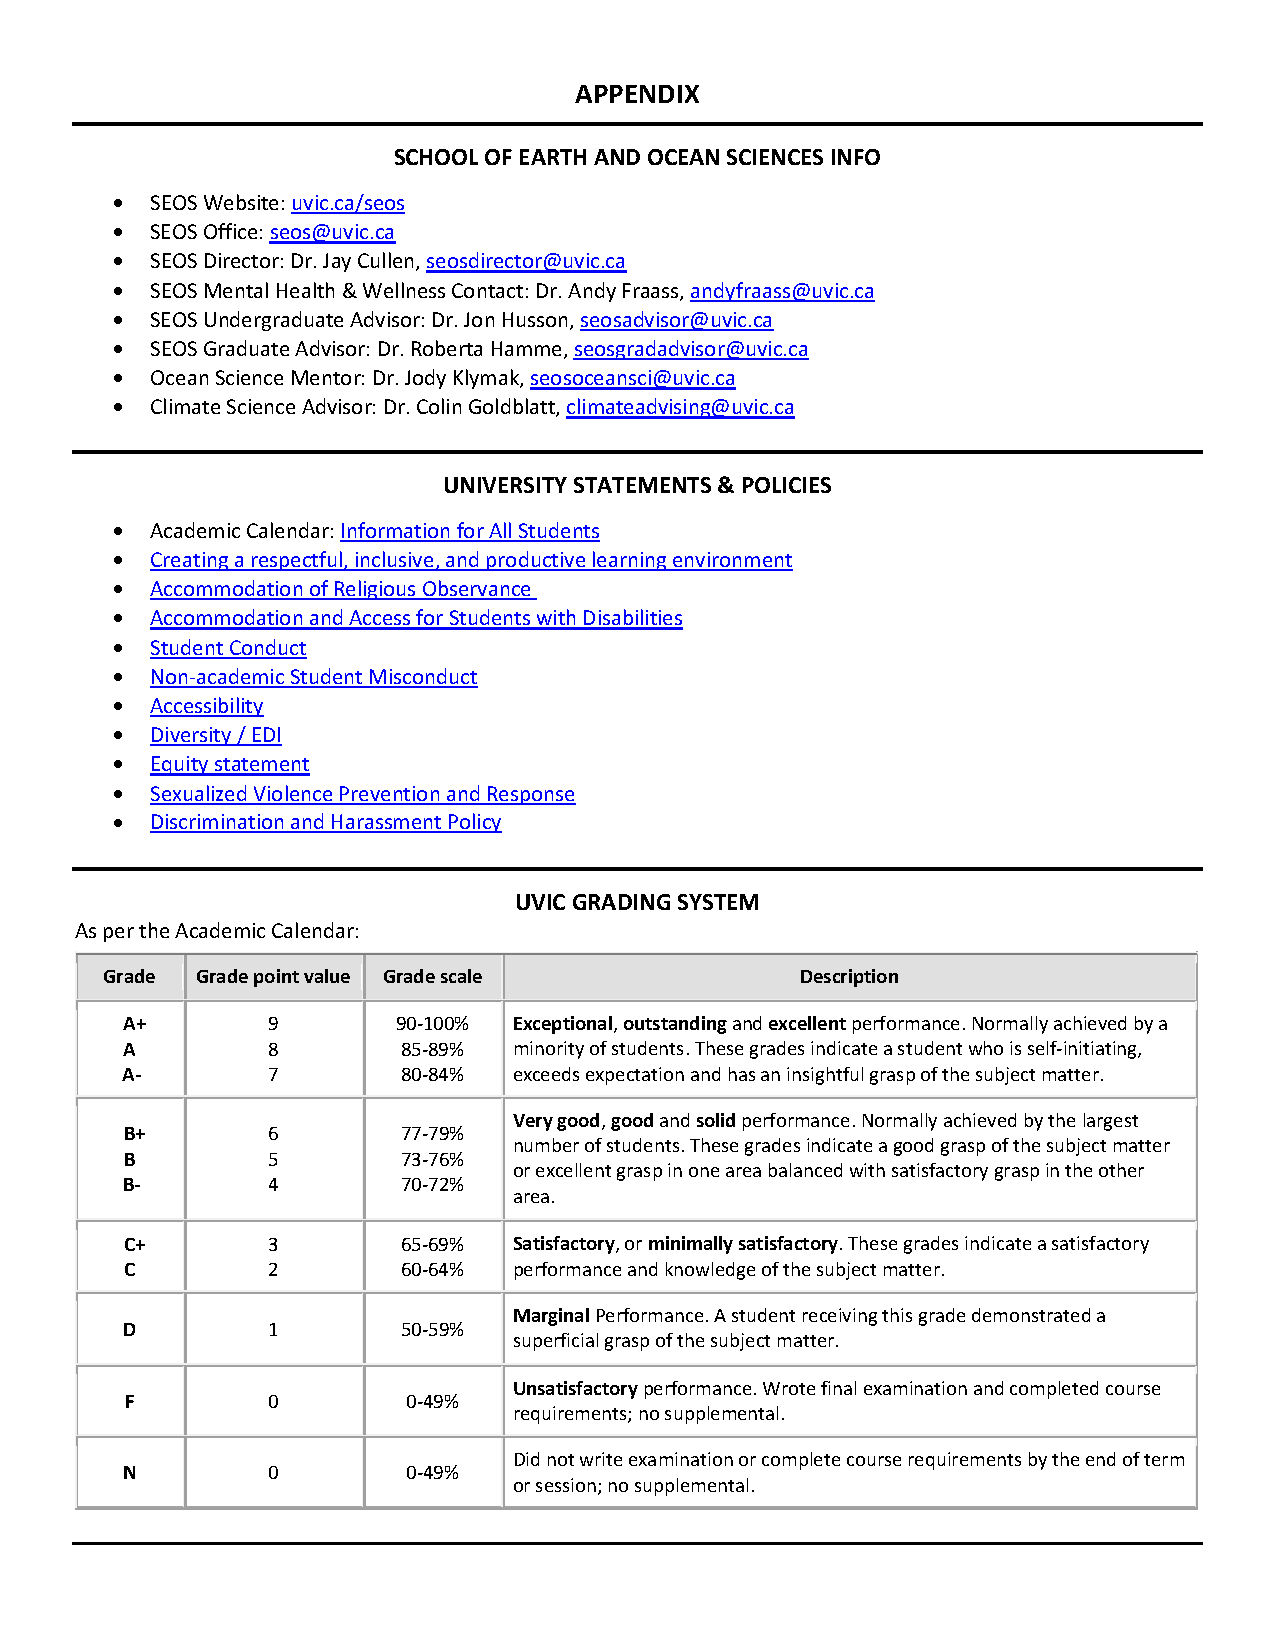
\includepdf[pages=-,pagecommand={},width=\textwidth]{Appendix.pdf}

\end{document}
